% !TEX TS-program = pdflatex
% !TEX encoding = UTF-8 Unicode

% This is a simple template for a LaTeX document using the "article" class.
% See "book", "report", "letter" for other types of document.

\documentclass[11pt]{article} % use larger type; default would be 10pt

\usepackage[utf8]{inputenc} % set input encoding (not needed with XeLaTeX)

%%% Examples of Article customizations
% These packages are optional, depending whether you want the features they provide.
% See the LaTeX Companion or other references for full information.

%%% PAGE DIMENSIONS
\usepackage{geometry} % to change the page dimensions
\geometry{a4paper} % or letterpaper (US) or a5paper or....
% \geometry{margin=2in} % for example, change the margins to 2 inches all round
% \geometry{landscape} % set up the page for landscape
%   read geometry.pdf for detailed page layout information

\usepackage{graphicx} % support the \includegraphics command and options

\usepackage[parfill]{parskip} % Activate to begin paragraphs with an empty line rather than an indent

%%% PACKAGES
\usepackage{booktabs} % for much better looking tables
\usepackage{array} % for better arrays (eg matrices) in maths
\usepackage{paralist} % very flexible & customisable lists (eg. enumerate/itemize, etc.)
\usepackage{verbatim} % adds environment for commenting out blocks of text & for better verbatim
\usepackage{subfig} % make it possible to include more than one captioned figure/table in a single float
% These packages are all incorporated in the memoir class to one degree or another...
\usepackage{amsmath}

%%% HEADERS & FOOTERS
\usepackage{fancyhdr} % This should be set AFTER setting up the page geometry
\pagestyle{fancy} % options: empty , plain , fancy
\renewcommand{\headrulewidth}{0pt} % customise the layout...
\lhead{}\chead{}\rhead{}
\lfoot{}\cfoot{\thepage}\rfoot{}

%%% SECTION TITLE APPEARANCE
\usepackage{sectsty}
\allsectionsfont{\sffamily\mdseries\upshape} % (See the fntguide.pdf for font help)
% (This matches ConTeXt defaults)

%%% ToC (table of contents) APPEARANCE
\usepackage[nottoc,notlof,notlot]{tocbibind} % Put the bibliography in the ToC
\usepackage[titles,subfigure]{tocloft} % Alter the style of the Table of Contents
\renewcommand{\cftsecfont}{\rmfamily\mdseries\upshape}
\renewcommand{\cftsecpagefont}{\rmfamily\mdseries\upshape} % No bold!

\usepackage{algpseudocode}
\usepackage[section]{algorithm}

\usepackage{hyperref}

%%% END Article customizations

%%% The "real" document content comes below...

\title{Identification over encrypted Channels}
\author{Niemczyk, Brandon \\  {\footnotesize {\tt brandon.niemczyk@hp.com, HP DVLABS}} \and Rao,Prasad \\ {\footnotesize {\tt prasad.rao@hp.com, HP LABS}}} 
%\date{} % Activate to display a given date or no date (if empty),
         % otherwise the current date is printed 

\numberwithin{equation}{section}

\begin{document}
\maketitle
\section{Living Document}

This paper is a living document, please grab the latest version from \\
https://raw.githubusercontent.com/bniemczyk/pacumen/master/paper/pacumen.pdf

\section{Introduction}

The ability to dynamically classify and identify the entities behind
network traffic could help us with various network activities.  These
activities include IP network engineering with network provisioning
and network management. This ability is especially important for
surveillance for policy compliance and security.

Today's techniques, when applied to traffic that is not hidden rely on
the visibility of packet headers, port numbers and the protocol, and
stateful reconstruction of sessions.  These cues disappear when ssh,
SSL or other tunneling mechanisms are used to hide traffic. Whether
the hiding is legitimate or not, it is advantageous to identify
information about encrypted traffic. Enterprises might proscribe
service providers that either allow policy violations or cause a
competitive disadvantage.  Campus networks could desire to prevent
games from clogging up the available bandwidth.  From the point of
view of a network provider, better classification and understanding of
traffic could allow better traffic shaping. Entities interested in
policy enforcement could also derive more meta data by such analysis.

We shall use the term \emph{identification problem} to mean the act of
identifing traffic behind encrypted channels.  There are several
published techniques resulting from many years of research in order to
classify traffic -- most of them rely on machine learning.


We are releasing a simple tool that we call {\tt pacumen}, that relies
on simple, easily collectible features in order to solve the
\emph{identification problem}. This tool is intended to be be easy to
use, and when compared to the academic approaches, need smaller amount
of data for training and lesser user intervention for it to
function. Additionally, as this tool is released as an open source
project on {\tt github}, we expect users to extend this tool and
contribute to its growth.  Our main purpose in this exercise to gain
insight and understanding to the phenomenon of hiding traffic behind
encrypted tunnels and the process of applying machine learning
techniques in an attempt to uncover them.  This work should both lead
to better techniques on both sides of this hide-and-seek game. Lastly,
we present some experiments and their results to validate {\tt
  pacumen}.

\section{Related Work/Prior Research}
Due to the fundamental nature of the \emph{identification problem}
there has been much work over a long period of time
that has explored the identification of applications/traffic
types over encrypted channels or at least in a payload agnostic manner. 
Table~\ref{tab1} illustrates a selection of this work. 

We cite two attempts at comparing various machine learning algorithms
in conjunction with several features to solve the \emph{identification 
problem}. 
Lim \emph{et al} \cite{lim2000comparison} compare twenty-two decision
tree, nine statistical, and two neural network algorithms on
thirty-two datasets with respect to classification accuracy, training
time, and (in the case of trees) number of leaf nodes.  They measure
classification accuracy by mean error rate and mean rank of error
rate.  They state that most of these algorithms perform similarly with
a statistical, spline-based, algorithm called Polyclass working
slightly better than other algorithms.  Another statistical algorithm,
logistic regression, is second with respect to the two accuracy
criteria.  They find that the most accurate decision tree algorithm is
Quest with linear splits, which ranks fourth and fifth, respectively.
Although spline-based statistical algorithms tend to have good
accuracy, they also require relatively long training times. Polyclass,
for example, is third last in terms of median training time. It often
requires hours of training compared to seconds for other
algorithms. The Quest and logistic regression algorithms are
substantially faster. Among decision tree algorithms with univariate
splits, C4.5, Ind-Cart, and Quest have the best combinations of error
rate and speed. But C4.5 tends to produce trees with comparitively a
large number of leaves.
Alshamarri \emph{et al} \cite{alshammari2009machine} compare AdaBoost,
Support Vector Machines, Naive Bayesian, RIPPER and C4.5.  They find
that C4.5 is the best of these.



Some techniques such as the one by Bernaille \emph{et
  al}\cite{bernaille2006traffic} require very few features to be
collected -- only the first five packets are used. The number five was
arrived by trying different number of packets, and different numbers of 
clusters and finding the pair $\langle 5,50 \rangle$ to yield the best
results.


 Karagiannis
\emph{et al} \cite{karagiannis2005blinc} enhance their classification
mechanism with some social, functional and application level
information, and obtain good accuracy.  

Roughan \emph{et al}
\cite{roughan2004class} perform classification for the purpose of
quality of service(QOS) maintenance.


\begin{table}[htbp]
\begin{small}
\begin{tabular}{||p{30mm}|p{35mm}|p{25mm}|p{25 mm}||}
\hline
Authors & ML Technique & Data, Quantity, Features & Accuracy \\
\hline
\hline
Williams et al \cite{williams2006preliminary}  & 
(i) Baysesian with discretized featured (ii) C4.5 (iii) Naive Bayes (iv) Naive Bayes Tree.   Feature reduction using correlation and consistency. 
Filter vs. wrapper models.  Sampling to limit number of flows. 

 &auckland-vi-2001061{1,2}  leipzig-ii-20030221, nzix-ii20000706 4000 Flows per application class ; 22 Features & $> 80 \%$ \\
\hline
%------------------------------------------------------------------
McGregor \emph{et al} \cite{mcgregor2004flow} &  Expectation Maximization(EM)   & packet length, inter-arrival time and flow duration. & NA, unsupervised\\
%--------------------------------------------------------------------------------------
%\hline
%\cite{dunnigan2000flow} & PCA to detect consistent statistical patterns & &  \\
%-----------------------------------------------------
\hline
Zander \emph{et al}\cite{zander2005automated} &  Greedy Forward Feature Search and EM   & subset of Table~\ref{flfeatures} &  average of $86.5\%$\\
%-----------------------------------------------------
\hline
Roughan \emph{et al} \cite{roughan2004class} &  Nearest Neighbor (NN) and linear discriminate analysis (LDA) into interactive or  transactional& packet, flow, connection, intra-flow, multi-flow & 90s \\
%-----------------------------------------------------
\hline
Moore \emph{et al} \cite{moore2005internet}  & Naive Bayes Classifier, Correlation based  selection of stronger features  &  248 flow features -- packet length, inter-arrival times & $> 65 \%$ per flow. $70 - 97 \%$ with Kernel density estimation and  and $> 90\%$ with FCBF Filtering  \\
%---------------------------------
\hline
Karagiannis {\em et al} \cite{karagiannis2005blinc}&graph-based& social, functional, application& $> 95 \%$\\
\hline
Bernaille {\em et al} \cite{bernaille2006traffic}&  K-means clusterting & First 5 packets&$> 80 \%$  \\
\hline
Lim \emph{et al}\cite{lim2000comparison} &  33 algorithms &  32 data sets &\\
\hline
Alshammari, Zincir-Heywood \cite{alshammari2009machine}& 5 algorithms & ssh v.s skype features in Table~\ref{flfeatures} on old standard data &  $>90\%$ \\
\hline
Zhang {\em et al} \cite{zhang2013robust}& k-NN, Bayesian, random forest & number of packets, bytes transferred, packet size, inter-packet time & variable\\
\hline
Branch {\em et al}\cite{branch2009rapid}& C4.5 & Skype identification.  Packet lengths, inter arrival times, large v/s small packets& $>98\%$\\
\hline
\end{tabular}
\end{small}
\caption{\label{tab1} Related Machine Learning Approaches Compared}
\end{table}




\begin{table}[htbp]
\begin{tabular}{|l|l|}
\hline
 Protocol &   Duration of the flow\\
\hline
\# Packets in forward direction & \# Bytes in forward direction\\
\# Packets in backward direction & \# Bytes in backward direction\\
Min forward inter-arrival time  & Min backward inter-arrival time\\
Std deviation of forward interarrival
times &
Std deviation of backward interarrival
times\\
Mean forward inter-arrival time & Mean backward inter-arrival time\\
Max forward inter-arrival time &  Max backward inter-arrival time\\
Min forward packet length & Min backward packet length\\
Max forward packet length & Max backward packet length\\
Std deviation of forward packet
length &
Std deviation of backward packet
length\\
Mean backward packet length &Mean forward packet length\\
\hline
\end{tabular}
\caption{\label{flfeatures}Typical feature set for a ML algorithm}
\end{table}

The results of Table~\ref{tab1} would perhaps suggest that it is easy
to get accuracies of greater than $80\%$ while solving the identification
problem using machine learning techniques.  While we have had similar
successes in attempting to identify Skype against non-Skype, we have
not had similar successes with other classification attempts over
browser-based applications such as gmail.

Absorbing the work that went behind all these papers gave us much better insight and intuition into the nature of the identification problem and the techniques to solve it than if we were to attempt solving it from scratch. 

\section{A quick introduction to Machine Learning}

Given that this problem has been addressed using machine learning techniques,
it is fruitful to introduce these properly (beyond presenting a laundry list
of machine learning algorithms). In his book \cite{mitchell1997machine}, Tom Mitchell defines \emph{learning} as:
A computer program is said to {\bf learn} from experience $E$ with
respect to some tasks $T$ and some performance measure $P$ if its
performance at tasks in $T$ improves with $E$.

When using machine learning for the act of assigning entities to classes,
the result of learning is a \emph{classifier} which can be 
applied to instances not seen during training.

Our main goal, while solving the identification problem is not to
debate the meaning of the word \emph{learning} but to find algorithms
and techniques that satisfy the above definition and to devise some
ourselves.

The act of designing a machine learning system incudes firstly the
design or choice of the training experience. Secondly, we must choose
or design a target function that helps us with the act of classification.
Thirdly, we need to choose a representation of this target function. 
We need to arrive at approximation schemes to evaluate this target function
for values not in the training set. We will describe how we performed
all of  these steps listed above in the next section.

\subsection{Issues while designing machine learning systems}
The list of Machine Learning algorithms continues to grow and some of
them are being used heavily in the real world.  Understanding the
appropriateness of these algorithms to the problem being solved, and
following up this understanding with a decision of which algorithm to use
is difficult.  Also, the decision of having to design a new algorithm is
not an easy one, and needs justification -- often by appealing to 
the special features of the problem at hand.

It is often asserted in literature that a large amount of data with
simple algorithms outperforms sophisticated algorithms with smaller
amounts of data.  The central question here is: \emph{How much
  training data is sufficient?} How can we quantify the confidence 
in the learning done on the training data?

How much can we use prior knowledge in these systems. For instance is it
OK to pre-process data -- by ignoring some particular features, even if the 
knowledge guiding this decision is approximate?

When should re-training be done?  Should we do the same kind of training
as we did before, or should we modify the training -- say, by adding/deleting
features? 

What form should the classifier take? Should we let the learning system decide this? 

\subsection{Performance Issues}
Sophisticated machine learning algorithms allow parameterization of
the extent to which they will fit the model to the training data. It
is easy to fall into the trap of overfitting the data -- in which case
results in the laboratory look very good. These models do not often 
perform as well on real world data.  

In our case, the application of standard machine learning algorithm
such as \emph{BayesianLogisticRegression} to the problem of distinguishing
Skype from everything else had a \emph{precision} of $1$ which means that
it had no false positives and a \emph{recall} of $0.872$.  We are in the
process of determining the extent of overfitting in this and other good
results by applying the same technique to 10x the amount of data.  

\section{Our Approach}

Our approach is to break the stream up by time buckets and try various weak classifiers on buckets and then adjust our confidence over time.  The reason for using time based windows instead of a set amount of packets is that intuitively there is a better chance of identifying the application even if it is mixed with traffic from other applications on the tunnel. %(\ref{breakdown}).  
See \ref{windowclass} for classifying each time window and \ref{bayes} for information on updating the confidence over time.

%I am assuming that it reads better without the subsection. Feel free to revert.
%\subsection{Features}
We looked at two primary \emph{features} - packet size counts and timing between packets.  In our experience the timing was too noisy for accurate classification, but the packet size counts and relations between them are very useful.  And we can implicitly include some timing information by generating our feature vectors as a function of time.  So what we do is generate a single 65536 dimension feature vector where each dimension is a count of the number of packets with a size that is the same as the "number" of that dimension.

%\subsubsection{An example of where classifying a set amount of packets will break down}
%\label{breakdown}

As an illustration, if you take say 100 packets and treat that as your feature vector, and the user is 1) using skype and 2) watching a youtube video.  It is likely you will get no traffic for skype or at least not get consistent numbers of packets in that 100 length sequence due to being overwhelmed with video data.  On the other hand  in a 10 second window you can expect a certain amount of traffic from any particular application you are looking to identify, and our feature selection will ideally discard most of the noise.

Figure ~\ref{fig:bucket} displays a simple workflow with a 10 second window that saw 6 packets, 3 of which were sizes that the classifier deems relevant.

\begin{figure}
  \centering
  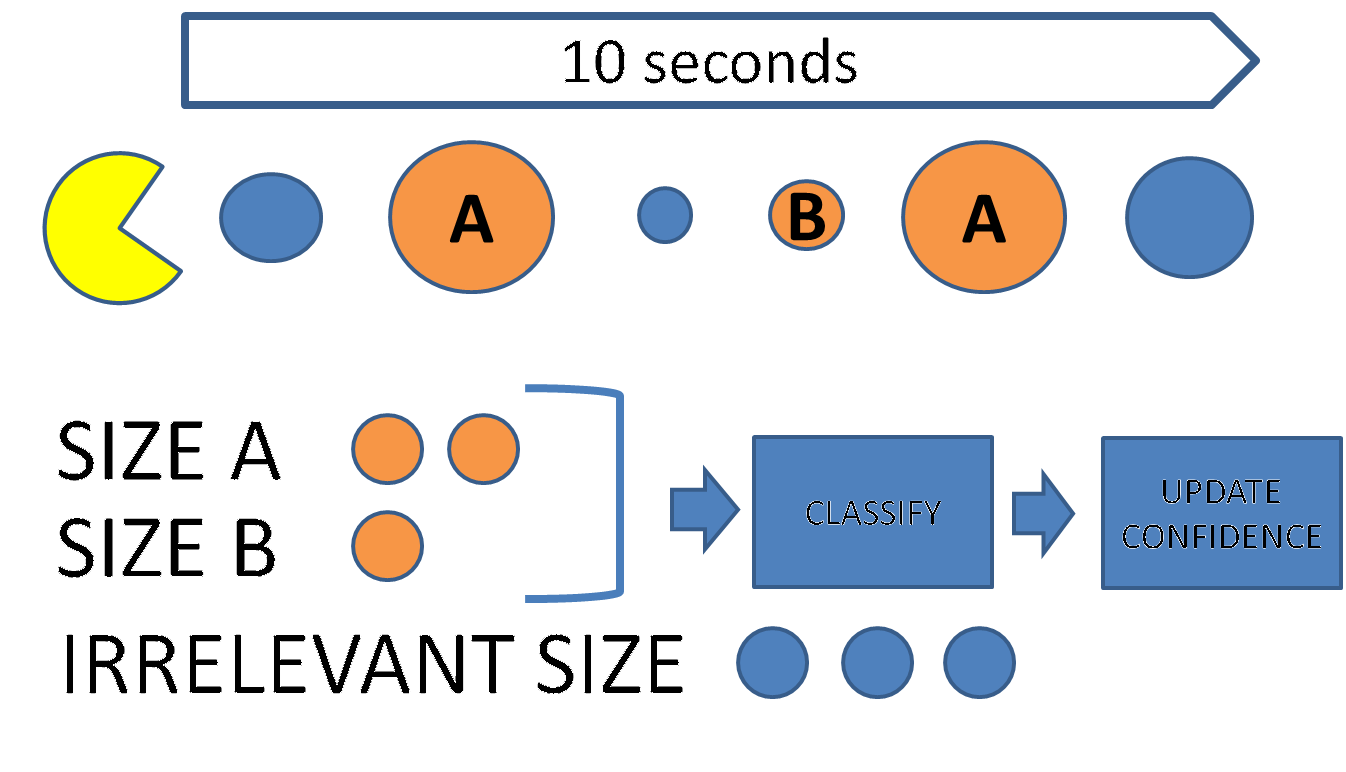
\includegraphics[width=0.9\textwidth]{bucketill.png}
  \caption{Illustration of bucketing sizes for a time window}
  \label{fig:bucket}
\end{figure}


\subsection{Algorithms used to classify 10 second windows of traffic}
\label{windowclass}

In order to be able to easily update our confidence using section ~\ref{bayes} our window classifier needs to return an estimate of the probability of the feature vector for both our negative and positive classes.  We should emphasize that
it is not  a probability that it belongs to the positive class.

\begin{description}

  \item[Likelihood function] Assume traffic is generated by a mixed gaussian and estimate the density function using the multi-variate normal likelihood function (Equation ~\eqref{eq:likelihood}).

  \item[Decision trees] See section ~\ref{dtree}.  This performs significantly better than the Likelihood function.

    \begin{flalign}
      \label{eq:likelihood}
      & L(\mathbf x) = e^{-\frac{1}{2} \ln(|\Sigma|) - \frac{1}{2}(\mathbf x - \mathbf \mu)^T \Sigma^{-1}(\mathbf x - \mathbf \mu) - \frac{k}{2} \ln(2 \pi)} & \\ \nonumber \\
      & \textbf{where} & \nonumber \\
      & \mathbf x = \text{column feature vector} & \nonumber \\
      & \mu = \text{Sample mean column vector} & \nonumber \\
      & \Sigma = \text{Sample covariance matrix} & \nonumber \\
      & |\Sigma| = \text{determinant of $\Sigma$} & \nonumber \\
      & k = \text{number of dimensions (65536)} & \nonumber
    \end{flalign}
\end{description}


\subsubsection{Decision Tree Algorithm}
\label{dtree}

\begin{figure}
  \centering
  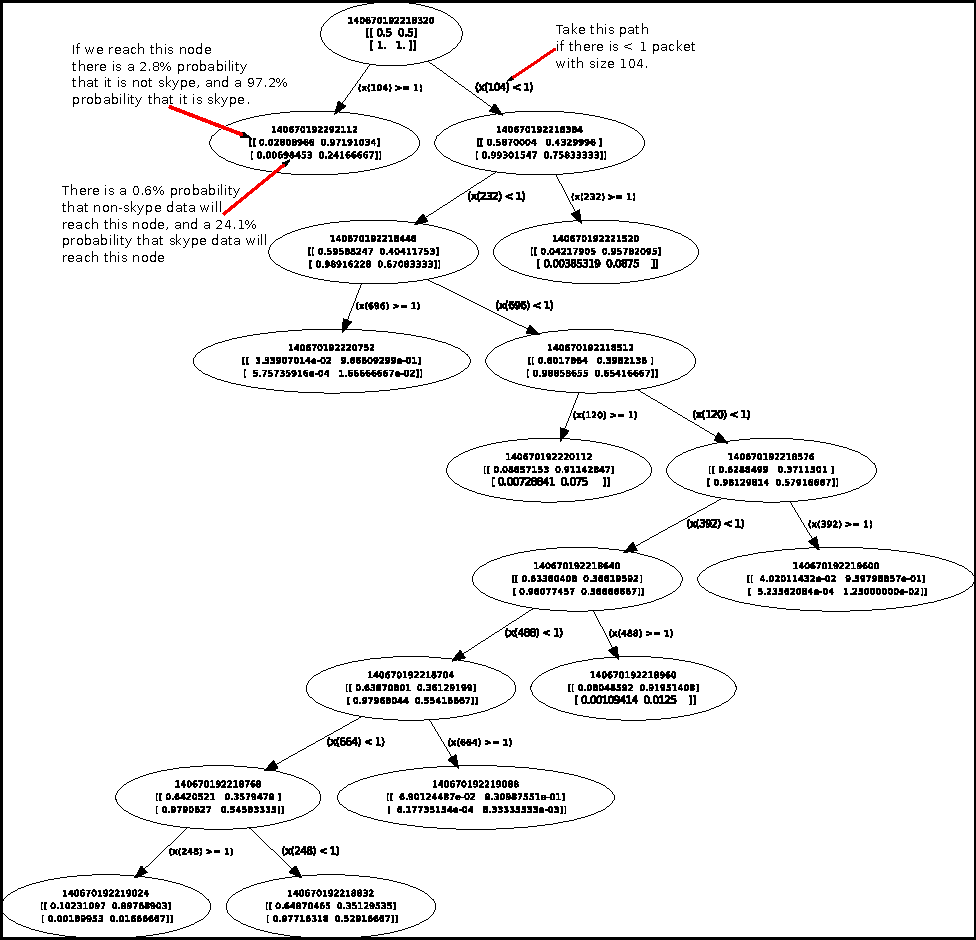
\includegraphics[width=0.9\textwidth]{sshdtree.pdf}
  \caption{Example Skype/SSH decision tree}
  \label{fig:dtree}
\end{figure}

See Figure ~\ref{fig:dtree} for an example of a Decision Tree that we would like to create.

Algorithm ~\ref{alg:dtree} describes the decision tree creation algorithm in pseudocode.  These trees give much better accuracy than the likelihood function and in fact get perfect accuracy with Skype, which most of the existing work has used.  The bias parameter is important to help avoid overfitting, and can be set by the user.  Additionally, the tools provided can search for the best bias.

\begin{algorithm}
  \caption{Decision Tree Creation Algorithm}
  \label{alg:dtree}
  \begin{algorithmic}
    \Function{SelectFeatureAndCutoff}{$data,bias$}
      \State $col \gets \bot$
      \State $cut \gets \bot$
      \State $max \gets -\infty$

      \ForAll{$\{column,thresh | column,thresh \in features \times values\}$}
        \State $igain \gets \text{information gain ratio using column and thresh}$
        \\\\
        \Comment{We use the $bias$ parameter to bias our selection to column/thresh pairs that look for a decrease in the probability of the positive class on the $<$ side, this is so that we do not learn that a protocol "will not have these sizes"}
        \\\\

        \State $score \gets {(P(col >= thresh | positive) * \frac{P(col >= thresh | positive)}{P(col >= thresh | negative)} * igain^{bias})}^\frac{1}{2 + bias}$
        \If{$score > max$}
          \State $max \gets score$
          \State $col \gets column$
          \State $cut \gets thresh$
        \EndIf
      \EndFor

      \State \Return $col, cut$
    \EndFunction
    \\\\
    \Function{ExpandNode}{$data,bias$}
      \State $p \gets \text{probability of positive class given } data$
      \If{$p < \epsilon \lor p > 1 - \epsilon$}
        \State \Return
      \EndIf
      \State $f,c \gets \text{SelectFeatureAndCutoff(}data,bias\text{)}$
      \State $low \gets \{ x | x \in data \land x[f] < c \}$
      \State $high \gets \{ x | x \in data \land x[f] >= c \}$
      \State ExpandNode($low$)
      \State ExpandNode($high$)
    \EndFunction
    \\\\
    ExpandNode(training data)
  \end{algorithmic}
\end{algorithm}

\subsection{Using Bayes Rule to update our confidence}
\label{bayes}

\paragraph
For each network stream we maintain a probability that the stream contains data from our positive class ($P(CLASS|DATA)$).  For every 10 seconds of data we then create a feature vector and estimate $P(DATA|CLASS)$ for both the positive and negative classes using either the likelihood function or decision trees.  Once we have this estimate we can update our stored prior (confidence if you prefer) using Bayes' Rule (Equation \eqref{eq:bayes}).

\begin{equation}
  \label{eq:bayes}
  P(CLASS|DATA) = \frac{P(DATA|CLASS) P(CLASS)}{\Sigma_{C \in CLASSES}{P(DATA|C) P(C)}}
\end{equation}

\section{Experiments and Results}
We collected the data using the {\tt --nflog} option in iptables, for outbound packets only. 
We extracted the features using the python wrapper to libcap --{\tt scapy} in linux and {\tt winpcapy} in windows.  

The pacumen tool can be run directly within a {\tt iPython} notebook and setting a variable to point to the directory with the pcap files. 
In order to run algorithms in Weka\cite{hall2009weka} we provide a converter. 
\section{Discussion}

%Metrics that we use to evaluate our techniques:

%$accuracy = \frac{Number\ of\ Correctly\ classified\ instances}{Total\ number\ of\ instances}$
We resort to standard measures of precision, recall and f-measure to
demonstrate the efficacy of our approach.

\[precision = \frac{Number\ of\ Correctly\ classified\ instances}{Total\ number\ of\  positive\ classifications}\]


\[recall = \frac{Number\ of\ Correctly\ classified\ instances}{Total\ number\ of\ class\ members}\]

\[f-measure = 2 . \frac{precision.recall}{precision + recall}\]



%\subsection{Use of Standard Machine Learning Algorithms}
We ran our experiments on our machine learning algorithms and also on
standard machine learning algorithms in Weka. Table \ref{tbl-std}
shows the result.

The results are comparitively worse for the classes {\tt firefox.gmail} and {\tt firefox.linkedin}.  The extra rows {\tt gmail}
and {\tt linkedin} were created by combining the firefox and chrome versions of these classes.   It can be observed that
this union yielded better results, leading to the conclusion that the firefox and the chrome versions of the classes were often mistaken for one another. 

% The comparitively better results we see in the row for skype is either a reflection of
% the fact that skype being a standalone entity rather than a web-page based one,
% makes it easy to be distinguished, or we were just plain lucky -- by the time of
% the black hat event we will resolve this question by subjecting pacumen to 
% 10x the amount of data. We will wait till then to arrive at a detailed 
% comparison of our machine learning technique with standards ones from Weka.



\begin{table}[h]
\begin{small}
\begin{tabular}{|l|l|l|l|l|l|l|l|l|l|l|l|l|}
\hline
& \multicolumn{3}{|c|} {J48} & \multicolumn{3}{|c|} {LADTree} &  \multicolumn{3}{|c|} {BLR} & \multicolumn{3}{|c|} {Our Tree} \\
\hline
& P & R & F & P & R & F & P & R & F & P & R & F \\
\hline
chrome.facebook  & .92 &	.79 &	.85 & .87 &	.82 & .84 & .85 & .70 &	.77 & .70 & .96 & .81\\
chrome.gmail     & .64 &	.32 &	.43 & .60 &	.38 & .46 & .59 & .54 &	.56 & .38 & 1.0 & .55\\
chrome.linkedin  & .51 &	.56  &	.54 & .63 &	.40 & .49 & .78 & .72 &	.75 & .95 & .43 & .59\\
firefox.facebook & .84	& .64 &	.72 & .86 &	.73 & .79 & .88 & .67 &	.76 & .33 & 1.0 & .50\\
firefox.gmail    & .30 &	.15 &	.21 & .68 &	.34 & .46 & .88 & .67 &	.76 & .18 & 1.0 & .31\\
firefox.linkedin & .30 &	.15 &	.21 & .67 &	.31 & .42 & .82 & .35 &	.49 & .50 & 1.0 & .66\\
linkedin         & .71 &	.45 &	.64 & .67 &	.47 & .55 & .69 & .57 &	.62 & --   & --   & --  \\
gmail            & .86 &	.50 &	.78 & .76 &	.72 & .74 & .80 & .78 &	.79 & --   & --   & --  \\
skype            & .89 &	.90 &	.90 & .95 &	.90 & .92 & 1.0 & .87 &	.93 & 1.0 & 1.0 & 1.0\\
\hline
\end{tabular}
\end{small}
\caption{\label{tbl-std}Results of running some standard machine learning algorithms in Weka upon our data. The columns P,R,F stand for precision, recall and f-measure respectively. BLR stands for Bayesian Logistic Regression. }
\end{table}



%More text.
\bibliography{tunnelDetect}
\bibliographystyle{plain}
\end{document}
